\documentclass[11pt]{article}

\usepackage[letterpaper,margin=1in]{geometry}
\usepackage[T1]{fontenc}
\usepackage{lmodern}
\usepackage{microtype}
\usepackage{amsmath,amssymb}
\usepackage{booktabs}
\usepackage{tabularx}
\usepackage{array}
\usepackage{enumitem}
\usepackage{graphicx}
\usepackage{tikz}
\usetikzlibrary{arrows.meta,positioning,fit,calc}
\usepackage{xcolor}
\usepackage[numbers,sort&compress]{natbib}
\usepackage{url}
\usepackage[hidelinks]{hyperref}
\usepackage[nameinlink,noabbrev]{cleveref}
\usepackage{caption}

\definecolor{ngblue}{HTML}{17324D}
\definecolor{ngteal}{HTML}{2B7A78}
\definecolor{nggray}{HTML}{5D6871}
\definecolor{nglight}{HTML}{EEF4F3}

\hypersetup{
  pdftitle={Who Authored the Evidence? Actor--Evidence Coupling in AI-Assisted Software Acceptance},
  pdfauthor={Ben Huffer},
  pdfsubject={Evidence custody and actor--evidence coupling in AI-assisted software acceptance},
  pdfkeywords={coding agents, AI-assisted software engineering, evidence custody, actor--evidence coupling, independent review, software assurance}
}

\newcommand{\method}{Nuclear-grade Context Engineering}
\newcommand{\repo}{\texttt{FlyFission/nuclear-grade-context-engineering}}
\newcommand{\verdict}{\textsc{Verdict}}
\newcommand{\applyclearance}{\textsc{Apply-clearance}}
\newcommand{\etal}{\textit{et al.}}
\newcommand{\code}[1]{\texttt{#1}}

\setlist{nosep}
\setlength{\parindent}{0pt}
\setlength{\parskip}{0.45em}
\captionsetup{font=small,labelfont=bf}

\title{\textbf{Who Authored the Evidence?}\\
Actor--Evidence Coupling in AI-Assisted Software Acceptance}

\author{Ben Huffer\\
\small FlyFission Consulting Group\\
\small \url{https://github.com/FlyFission/nuclear-grade-context-engineering}}

\date{July 20, 2026\\\small v0.3 RC2 discussion preprint}

\begin{document}
\maketitle

\begin{abstract}
AI coding agents can implement changes, select tests, summarize evidence, and write the review narratives used to accept those changes within one coupled process. Existing controls address self-modification: an actor editing the gate intended to constrain it. They do not necessarily address \emph{evidence self-authorship}: an actor that leaves the gate untouched while authoring the evidence the gate consumes. A confident hallucination can clear every gate for which it also wrote the input.

This paper formulates acceptance of agent-assisted changes as a problem distinct from agent task performance. It contributes an agent-specific formulation of evidence self-authorship and a multidimensional profile for actor--evidence coupling across actor, context, mechanism, authority, and resource. A consequence-graded admissibility proposal uses that profile to constrain decisive evidence through externally versioned policy rather than a universal score. The formulation adapts established self-review, configuration-management, independent-verification, and assurance practice rather than claiming to replace them. A Git-native reference implementation shows that custody labels, coupling profiles, and decision state can be represented, exercised, and structurally linted. A twelve-scenario formative inspection supports iteration, not efficacy claims. The paper states a falsifiable prediction and proposes a preregistered comparison of actor-controlled evidence with a specifically defined separated-evidence condition.
\end{abstract}

\noindent\textbf{Keywords:} coding agents; AI-assisted software engineering; evidence custody; actor--evidence coupling; independent review; configuration management; software assurance.

\section{Introduction}
\label{sec:introduction}

Coding agents have moved beyond code completion. A single agent session may discover repository state, interpret requirements, edit source and prompts, change dependencies, invoke tools, select tests, write the review narrative, and recommend release. This concentration of activity is productive, but it also creates a control problem. If the agent's model of the task is wrong, the same error can propagate into the change, the evidence selected to support it, the explanation presented to a reviewer, and the release recommendation. The result can be internally coherent without being trustworthy.

Most context-engineering guidance is designed to improve task performance: select high-signal instructions, retrieve relevant knowledge, expose tools, retain state, compact long histories, and give agents effective interfaces \citep{mei2025context,anthropic2025context,yang2024sweagent}. Those mechanisms are necessary, but they do not by themselves answer five acceptance questions:

\begin{enumerate}
  \item What was the agent authorized to change or execute?
  \item Which claims must be true before the change is accepted?
  \item Who or what produced the evidence supporting those claims?
  \item Which decision does the evidence support?
  \item Which accepted state must remain under configuration control?
\end{enumerate}

We call the information required to answer those questions \emph{context for accountable acceptance}. This is not a replacement for performance-oriented context. It is a narrower specialization for trust-bearing decisions: decisions that affect users, persistent data, money, permissions, external systems, public claims, release state, or other protected outcomes.

This paper presents \emph{graded accountable acceptance}, instantiated by the open \method{} reference implementation \citep{flyfission2026repo}. Throughout, ``nuclear-grade'' denotes the project's engineering posture and professional lineage drawn from public high-consequence practice; it does not claim regulatory status, safety classification, formal assurance, or demonstrated efficacy.

\subsection{Contributions}

The paper makes one problem-formulation contribution, one modeling contribution, and one implementation contribution:

\begin{enumerate}
  \item \textbf{Evidence self-authorship formulation.} It translates established self-review concerns to agent-assisted software acceptance and distinguishes gate self-modification from control of the evidence path. The formulation predicts that, for plausible but wrong changes, reviewer detection will degrade when the change actor also controls decisive evidence. It is falsified if controlled studies show no meaningful detection difference, or if protected gates bound acceptance error equally well.
  \item \textbf{Actor--evidence coupling profile.} It defines five axes---actor, context, mechanism, authority, and resource---for exposing correlated failure that nominally separate roles can conceal. It proposes that consequence policy constrain admissible coupling for decisive evidence without collapsing the axes into an assurance ladder. Universal minimum profiles are not claimed; they remain versioned policy choices outside a candidate's writable record.
  \item \textbf{Open reference implementation.} It shows that custody labels, coupling profiles, and decision state can be represented with ordinary repository artifacts, exercised, and structurally linted. The checks expose declared custody and coupling; they do not authenticate identities, establish semantic adequacy or independence, or decide whether a profile satisfies a consequence policy. Lifecycle stages, packet files, risk tiers, verdict/apply-clearance, and templates are implementation primitives rather than standalone research contributions.
\end{enumerate}

The work does not claim invention of configuration management, independent verification, governed context, assurance cases, professional self-review, human approval gates, or operational decision authority. Its claim is a narrow agent-specific synthesis around evidence custody and coupling in software acceptance.

\section{Background and Related Work}
\label{sec:related}

\subsection{Context, repository instructions, and agent harnesses}

Context engineering spans retrieval, memory, tool use, state management, compaction, and evaluation \citep{mei2025context}. Anthropic emphasizes the smallest high-signal context, just-in-time retrieval, progressive disclosure, and structured state \citep{anthropic2025context}. Repository conventions such as \code{AGENTS.md} provide tool-neutral standing instructions \citep{agentsmd2025}; Spec Kit and related workflows make specifications, plans, and task records first-class inputs to coding agents \citep{github2026speckit,medin2025context}.

Long-running-agent harnesses retain progress, use Git history, work incrementally, and require end-to-end checks \citep{anthropic2025harness}. OpenAI's harness-engineering account describes a repository as the system of record, a concise instruction map, mechanical documentation checks, enforceable architecture, isolated worktrees, observability, and agent-to-agent review \citep{openai2026harness}. SWE-agent demonstrates that the agent--computer interface materially changes repository navigation, editing, test execution, and task performance \citep{yang2024sweagent}.

These sources establish repository legibility, durable state, specifications, executable feedback, and harness design as prior art. \method{} adds an acceptance-oriented layer: explicit authority, controlled surfaces, evidence obligations, evidence provenance, decision rights, residual risk, and closure state.

\subsection{Evaluation integrity}

SWE-bench Verified used human-screened tasks and tests outside the solving agent, providing a benchmark-level example of solver--evidence separation \citep{openai2024swebench}. OpenAI later stopped using the benchmark for frontier-model evaluation because contamination and flawed tests had weakened the judge itself \citep{openai2026noswebench}. This sequence is important: independent execution does not make evidence valid when the evaluator, data, or environment has degraded. Actor--evidence independence is therefore one control among several, not proof of correctness.

Empirical work on repository-level instruction files likewise cautions against equating more context with better outcomes. Gloaguen \etal{} report that \code{AGENTS.md}-style context did not generally improve task success and increased inference cost in their studied settings \citep{gloaguen2026agents}. The implication for this method is subtraction: standing instructions should contain unusual constraints and exact routes, while deeper material should load only when needed.

Professional independence and model-evaluation research supply closer lineage for the central failure formulation. The IESBA Code defines a self-review threat as evaluating or relying on one's own prior work \citep{iesba2026code}. LLM evaluators can recognize and favor their own generations, while related generator and judge models can exhibit preference leakage across inheritance and model-family relationships \citep{panickssery2024evaluators,li2025preference}. Human-factors research likewise distinguishes appropriate automation use from misuse, disuse, and abuse and documents automation bias in decision making \citep{parasuraman1997automation,skitka1999automation}. Evidence self-authorship is therefore not a claim to have discovered self-review or automation bias. It is an agent-specific acceptance formulation that extends the concern from model scoring to the tests, summaries, omissions, risk framing, and claims consumed by a software-change decision.

\subsection{Configuration management, independence, and assurance reasoning}

Configuration identification, change control, status accounting, baselines, assessment, and controlled acceptance are established disciplines \citep{doe2016cm,nrc2013rg169}. Secure-software and AI-risk frameworks further establish protected artifacts, provenance, governance, and risk-management processes, but do not by themselves prescribe actor--evidence separation for coding agents \citep{nist2022ssdf,nist2023airmf}. NASA and NRC guidance establish independent verification, validation, review, and audit as lifecycle practices \citep{nasa2022swe141,nasa2022assurance,nrc2013rg168}. NIST assessment guidance addresses separation of duties and independent assessment evidence \citep{nist2022assessment}. Tool accreditation and intended-use reasoning are likewise established ideas \citep{nasa2022swe136}.

Claims--argument--evidence structures are mature assurance concepts \citep{nist2022systems,omg2023sacm}. Recent work applies safety-case reasoning to frontier AI and explores language models as aids for finding defeaters \citep{buhl2024safetycases,gohar2024codefeater}. \method{} does not claim to replace a formal assurance case. It uses a deliberately thin repository-native chain: basis $\rightarrow$ claim $\rightarrow$ control $\rightarrow$ evidence or gap $\rightarrow$ decision.

Public high-consequence guidance also provides lineage for graded rigor, questioning assumptions, self-checking, peer checking, independent verification, turnover, and operational learning \citep{doe2009hpi}. The translation in this paper applies those ideas to software agents without importing regulatory classifications or claiming domain equivalence.

\subsection{Adjacent acceptance, governance, and provenance work}

Software Delegation Contracts are the closest coding-agent empirical comparison. They structure work around task, bounded authority, returned work package, and acceptance context. A controlled pilot of 64 agent runs and 192 condition-blinded model-based reviews found improved reviewability rather than correctness, at increased token and wall-clock cost \citep{schmalbach2026contracts}. Artifact-gate research likewise compares prompt-to-code, specification-driven, and artifact-aware delivery using synthetic tasks and deterministic evaluators \citep{ravuru2026artifact}. These works occupy broad claims over evidence bundles, artifact gates, and reviewability. The distinction here is the custody and coupling of decisive evidence rather than the existence of a structured package.

Governed AI-Assisted Engineering independently proposes graduated human oversight based on regulatory impact, customer proximity, reversibility, and data sensitivity, with required evidence artifacts \citep{kang2026gaie}. This overlaps consequence grading; the present paper does not claim novelty for oversight tiers. ContextNest formalizes governed knowledge supplied to agents through version identity, provenance, integrity, approved status, and point-in-time reconstruction \citep{sulpovar2026contextnest}. Xu \etal{} likewise propose a persistent governed-context abstraction with access control, provenance, traceability, and human verification roles \citep{xu2025everything}. These systems govern context eligibility and retrieval; this paper focuses on evidence and authority at acceptance of a candidate software state.

Runtime Governance for AI Agents models enforceable decisions over agent identity, partial execution path, proposed action, and organizational state \citep{kaptein2026runtime}. AgentBound composes delegated authorization, behavioral constitutions, and site action contracts before execution and emits verifiable governance receipts \citep{kaul2026agentbound}. These systems are adjacent to apply-clearance and authority surfaces. The provenance survey by Wang \etal{} connects claims, evidence, tool outputs, memory, actions, and outcomes as a process-accountability graph \citep{wang2026traces}. Zhang and Sun's Knowledge-Based Pull Requests separate knowledge acceptance from implementation integration across a trust boundary \citep{zhang2026kpr}. Together these works preclude broad novelty claims over governed context, evidence bundles, provenance, graduated oversight, runtime authorization, or decision separation.

Two recent review-oriented works further narrow the contribution. Pollner treats AI-generated test artifacts as candidates requiring risk-scaled human acceptance rather than self-validating evidence \citep{pollner2026oversight}. Ming \etal{} organize intent, success criteria, actions, completion claims, verification evidence, gaps, and rework constraints into a reviewable claim structure and report improved detection of hidden intent--completion gaps under controlled materials \citep{ming2026reviewability}. The acceptance-record schema in this paper is therefore an implementation mechanism, not an invention claim.

Industrial prior art is also substantial. Palantir's Ontology connects semantic objects to governed actions; ontology proposals support review and approval; and scenarios remain hypothetical until associated actions are applied under validation and permission controls \citep{palantir2026ontology,palantir2026proposals,palantir2026scenarios}. These capabilities preclude novelty claims over operational ontologies, controlled proposal/merge workflows, or separation of a modeled state from authority to apply it. The residual distinction is whether the actor producing a candidate also controls the decisive evidence path.

The residual specialization is narrower: evidence self-authorship as an agent-specific, falsifiable acceptance problem; a multidimensional profile of actor--evidence coupling; a consequence-dependent admissibility proposal; and an open Git-native reference pattern. \Cref{tab:boundary} summarizes that boundary.

\begin{table}[t]
\centering
\caption{Contribution boundary.}
\label{tab:boundary}
\small
\begin{tabularx}{\textwidth}{>{\raggedright\arraybackslash}p{0.28\textwidth} >{\raggedright\arraybackslash}p{0.27\textwidth} X}
\toprule
Concept & Status & Treatment in this paper \\
\midrule
Context management, repository instructions, staged specifications & Established or adjacent & Credit prior work; no invention claim \\
Configuration management, baselines, graded rigor, IV\&V, assurance cases & Established & Use as public lineage; no domain-equivalence claim \\
Governed or accountable context & Adjacent work exists & Do not claim the broad category \\
Context for accountable acceptance & Problem boundary & Define around trust-bearing decisions \\
Self-modification vs. evidence self-authorship & Agent-specific formulation & Ground in self-review and model self-preference; falsifiable prediction in \Cref{sec:research} \\
Actor--evidence coupling profile & Modeling contribution & Five non-ordinal axes grounded in IV\&V, separation of duties, and common-mode failure \\
Controlled agent operating envelope & Implementation concept & Treat behavior-driving surfaces as configuration \\
Verdict vs. apply-clearance & Established-adjacent implementation primitive & Adapt decision authority to the repository workflow \\
Git-native acceptance record & Implementation vehicle & Demonstrate feasibility, not efficacy \\
\bottomrule
\end{tabularx}
\end{table}

\section{Problem Formulation}
\label{sec:problem}

\subsection{Trust-bearing changes}

Let $c$ be a candidate change to code, configuration, prompts, models, permissions, data policy, tests, or release state. A change is \emph{trust-bearing} when accepting it commits an organization to an externally meaningful or difficult-to-reverse state. Examples include widening an agent's tool permissions, changing a payment path, altering data retention, changing a model or evaluation baseline, or publishing an assurance claim.

Acceptance requires more than a successful execution trace. The method uses an \emph{acceptance-record schema} with eight fields: intent; discovered state; authority; claims; evidence and provenance; verdict and residual-risk disposition; accepted baseline; and revalidation or operational triggers. This is a record schema, not a proof system.

Let $\pi$ be a versioned consequence policy external to the candidate record. For consequence class $k$, acceptance is permitted only when the required fields for $k$ are present, each decisive claim has evidence whose coupling profile satisfies $\pi(k)$, unresolved gaps have an authorized disposition, and the verdicting actor has acceptance authority. Application additionally requires current apply-clearance. This paper proposes that predicate but does not define one universal $\pi$: organizations must state and protect their required profiles, decisive-claim rules, exceptions, and expected packet mode outside the surfaces a change actor may rewrite. A baseline loses reliance when a recorded trigger occurs, its evidence expires, or a behavior-driving surface changes beyond the accepted envelope. These predicates make omissions and invalid transitions inspectable without implying mathematical assurance.

\subsection{The evidence self-authorship failure mode}

Two related failure modes must be separated:

\begin{description}
  \item[Self-modification.] The actor can edit the control, test, policy, or threshold intended to constrain it.
  \item[Evidence self-authorship.] The actor cannot edit the gate but can author all evidence, summaries, risk framing, and conclusions consumed by that gate.
\end{description}

We use \emph{evidence custody} for effective control over an evidence item's generation, selection, transformation, execution environment, retention, and presentation. Provenance can identify where an artifact came from without showing who controlled those choices. Custody makes that control path explicit.

Locking a gate addresses self-modification. It does not address evidence self-authorship. An agent can leave a protected CI rule untouched while selecting favorable tests, summarizing incomplete output, omitting a failed condition, or writing the narrative on which a reviewer relies. The resulting gate is structurally separate but informationally coupled to the actor.

The central failure claim is therefore:

\begin{quote}
A confident hallucination can clear every gate for which it also wrote the input.
\end{quote}

This is not a claim that every agent-generated report is unreliable. Actor evidence is often useful and inexpensive. The point is that its provenance must be visible, and the required independence should scale with consequence.

\subsection{Threat model and control boundaries}

The primary threat is epistemic rather than adversarial: a well-intentioned but fallible actor produces a wrong change and a locally coherent account that repeats the same mistake. Evidence separation addresses correlated reasoning, selective testing, persuasive omission, and unsupported confidence. It does not by itself stop malicious behavior.

Other threats require different controls. Locked surfaces and least privilege address unauthorized modification and prompt-injected or compromised actors. Protected baselines address stale or silently changed configuration. Authenticated provenance addresses forged identity or rewritten evidence. Apply-clearance addresses changes in approvals, maintenance windows, external state, and rollback availability after technical acceptance. Human review addresses judgment but remains vulnerable to weak competence, incentives, time, and rubber-stamping. A compromised toolchain or colluding authority can defeat the pattern unless the deployment adds controls outside the actor's administrative domain.

\begin{figure}[t]
\centering
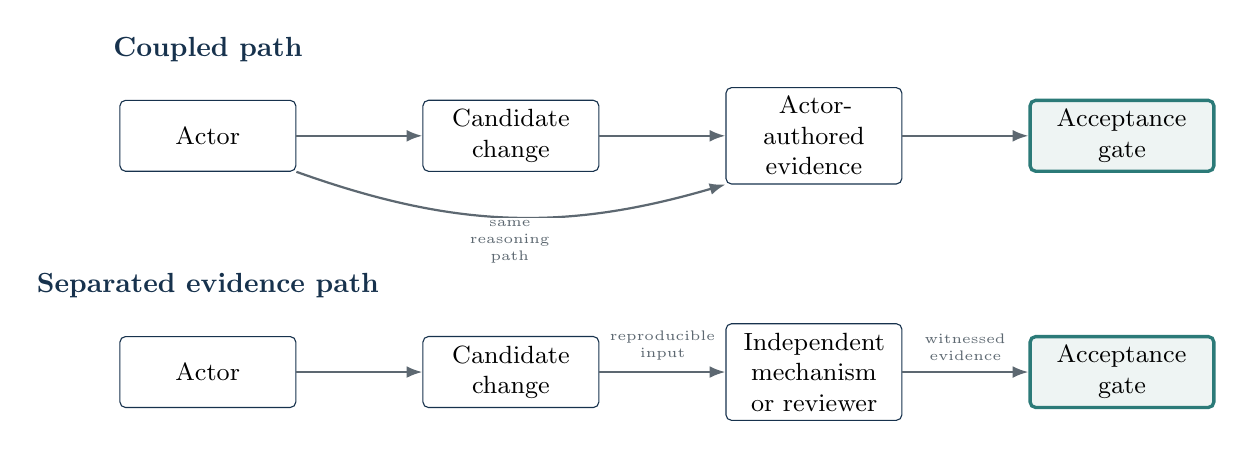
\begin{tikzpicture}[
  node distance=9mm and 16mm,
  box/.style={draw=ngblue, rounded corners=2pt, align=center, minimum height=9mm, text width=20mm, fill=white, font=\small},
  gate/.style={draw=ngteal, very thick, rounded corners=2pt, align=center, minimum height=9mm, text width=21mm, fill=nglight, font=\small},
  arrow/.style={-{Latex[length=2mm]}, thick, draw=nggray},
  label/.style={font=\tiny, text=nggray, align=center, fill=white, inner sep=1pt, text width=14mm}
]
\node[font=\bfseries, text=ngblue] (ca) at (0,2.0) {Coupled path};
\node[box] (actor1) at (0,0.9) {Actor};
\node[box, right=of actor1] (change1) {Candidate\\change};
\node[box, right=of change1] (evidence1) {Actor-authored\\evidence};
\node[gate, right=of evidence1] (gate1) {Acceptance\\gate};
\draw[arrow] (actor1) -- (change1);
\draw[arrow] (actor1.south east) to[bend right=18] node[below,label]{same\\reasoning path} (evidence1.south west);
\draw[arrow] (change1) -- (evidence1);
\draw[arrow] (evidence1) -- (gate1);

\node[font=\bfseries, text=ngblue] (sa) at (0,-1.0) {Separated evidence path};
\node[box] (actor2) at (0,-2.1) {Actor};
\node[box, right=of actor2] (change2) {Candidate\\change};
\node[box, right=of change2] (verify2) {Independent\\mechanism\\or reviewer};
\node[gate, right=of verify2] (gate2) {Acceptance\\gate};
\draw[arrow] (actor2) -- (change2);
\draw[arrow] (change2) -- node[above=1mm,label]{reproducible\\input} (verify2);
\draw[arrow] (verify2) -- node[above=1mm,label]{witnessed\\evidence} (gate2);
\end{tikzpicture}
\caption{Actor separation and evidence separation are different properties. A protected gate can still consume evidence coupled to the actor's reasoning path.}
\label{fig:coupling}
\end{figure}

\section{Implementation Vehicle: The Graded Acceptance Method}
\label{sec:method}

The coupling profile in \Cref{sec:independence} is the modeling contribution. This section introduces only the operational vocabulary needed to show where that profile enters acceptance; the lifecycle, modes, packet files, and operating envelope are implementation vehicles.

\subsection{Lifecycle}

The full lifecycle is

\begin{center}
\textsc{Question $\rightarrow$ Discover $\rightarrow$ Specify $\rightarrow$ Plan $\rightarrow$ Execute $\rightarrow$ Verify $\rightarrow$ Review $\rightarrow$ Decide $\rightarrow$ Baseline $\rightarrow$ Operate $\rightarrow$ Learn}.
\end{center}

The lifecycle is an information flow, not a meeting schedule or research contribution. A small change may represent several stages in a few lines; detailed mnemonics and role prompts remain in the reference repository.

\begin{figure}[t]
\centering
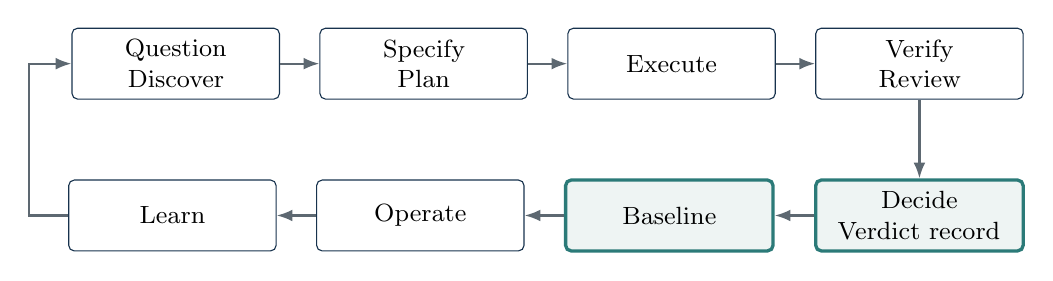
\begin{tikzpicture}[
  node distance=5mm,
  stage/.style={draw=ngblue, rounded corners=2pt, align=center, minimum height=9mm, text width=24mm, fill=white, font=\small},
  accept/.style={draw=ngteal, very thick, rounded corners=2pt, align=center, minimum height=9mm, text width=24mm, fill=nglight, font=\small},
  arrow/.style={-{Latex[length=2mm]}, thick, draw=nggray}
]
\node[stage] (q) {Question\\Discover};
\node[stage, right=of q] (sp) {Specify\\Plan};
\node[stage, right=of sp] (ex) {Execute};
\node[stage, right=of ex] (vr) {Verify\\Review};
\node[accept, below=10mm of vr] (de) {Decide\\Verdict record};
\node[accept, left=of de] (ba) {Baseline};
\node[stage, left=of ba] (op) {Operate};
\node[stage, left=of op] (le) {Learn};
\draw[arrow] (q) -- (sp);
\draw[arrow] (sp) -- (ex);
\draw[arrow] (ex) -- (vr);
\draw[arrow] (vr) -- (de);
\draw[arrow] (de) -- (ba);
\draw[arrow] (ba) -- (op);
\draw[arrow] (op) -- (le);
\draw[arrow] (le.west) -- ++(-5mm,0) |- (q.west);
\end{tikzpicture}
\caption{A compressed view of the acceptance loop; paired labels combine lifecycle stages with the decision record they produce. Rigor is concentrated at trust-bearing transitions rather than imposed uniformly during exploration.}
\label{fig:lifecycle}
\end{figure}

The operating principle is \emph{fast exploration, slow acceptance}. Agents may explore alternatives rapidly in a bounded workspace. A candidate becomes trust-bearing only when it is proposed for acceptance, release, application, or public reliance. Evidence and independence increase at that boundary.

\subsection{Graded modes}

A method for consequential work fails economically if it imposes the same ceremony on every change. \Cref{tab:modes} defines four levels. The mode is selected by authority, consequence, uncertainty, reversibility, and external trust rather than by diff size alone.

\begin{table}[t]
\centering
\caption{Consequence-graded artifact and review modes.}
\label{tab:modes}
\small
\begin{tabularx}{\textwidth}{>{\raggedright\arraybackslash}p{0.17\textwidth} >{\raggedright\arraybackslash}p{0.27\textwidth} >{\raggedright\arraybackslash}p{0.25\textwidth} X}
\toprule
Mode & Typical change & Artifact spine & Review expectation \\
\midrule
Administrative floor & Typo, comment, dead link; instantly reversible; no trust boundary & Commit message & Ordinary diff review \\
Quick & Local, reversible, easy to prove & Risk plus proof record & Reviewer can rerun proof \\
Standard & User-visible or lasting; dependency, data, permission, model, prompt, authority, or release impact & Risk, basis, plan, trace, verification, ship & Claims linked to evidence and explicit decision \\
Stronger subset & Severe, silent, difficult to reverse, externally trusted, or autonomous action & Standard plus only records earned by the risk & Independent evidence and named human authority scaled to consequence \\
\bottomrule
\end{tabularx}
\end{table}

Tripwires move a change upward when it introduces a trust boundary, irreversible action, destructive migration, permission widening, external claim, silent failure path, or material uncertainty. A successful graded method also permits de-escalation when the consequence and proof remain small. Where mode or minimum-profile compliance is mandatory, a protected policy owner must define the tripwires, expected mode, and $\pi(k)$ outside the candidate packet; a packet-local marker or PR-controlled validator cannot protect itself from downgrade.

\subsection{Change packets and context packs}

The Git-native unit is a change packet at

\begin{center}
\code{.nuclear/changes/<change-slug>/}.
\end{center}

A Standard packet uses six Markdown files to carry one acceptance record: risk and consequence; basis and claims; bounded plan and authority; trace links; verification and provenance; and verdict, residual risk, rollback, monitoring, and baseline triggers. The filenames are repository ergonomics, not separate constructs.

The packet does not replace issues, pull requests, tests, CI, or operations systems. It links those primary artifacts around one decision and prefers links to copied output. Its task-specific projection supplies an agent only the objective, authority, evidence obligations, stop conditions, source lineage, and open gaps needed for the current phase. The packet has failed when it becomes a repository summary, duplicated narrative, or AI-generated paperwork that no reviewer uses.

\subsection{Controlled agent operating envelopes}

Agent behavior depends on more than source code. The controlled configuration boundary may include system and repository prompts, model identifiers and settings, tool schemas, permissions, credential policy, evaluation cases, scoring rubrics, skills, retrieval rules, memory, context packs, and approval instructions. We call this the \emph{agent operating envelope}.

The term does not imply a formally qualified tool. It identifies behavior-driving surfaces that require versioning and revalidation when an organization relies upon them. A useful baseline records the accepted versions, intended use, evidence behind acceptance, known limits, residual gaps, and triggers that require a new check. This is a software-agent translation of established configuration-management and intended-use reasoning \citep{doe2016cm,nasa2022swe136}.

\section{Actor--Evidence Coupling and Independence}
\label{sec:independence}

Independence is not binary. A different process, agent label, or model call may share the same prompt, retrieved material, orchestrator, scoring rubric, and budget. The relevant question is whether the evidence path can fail differently from the implementation path.

An evidence item is therefore labeled with a five-axis profile $P=(a,c,m,u,r)$:

\begin{enumerate}
  \item \textbf{actor ($a$)}: whether a different actor performs or witnesses the check;
  \item \textbf{context ($c$)}: whether the verifier reconstructs the problem without inheriting the actor's narrative as fact;
  \item \textbf{mechanism ($m$)}: whether a different test, oracle, model family, tool, or human technique is used;
  \item \textbf{authority ($u$)}: whether the actor is unable to redefine scope, threshold, evidence sufficiency, or verdict; and
  \item \textbf{resource ($r$)}: whether the actor is unable to starve the verification budget or suppress its output.
\end{enumerate}

Each axis records \emph{coupled}, \emph{partially separated}, or \emph{separated}, with a short basis. The axes are analytic lenses, not presumed causally independent variables: one shared orchestrator, prompt, budget, or policy owner may couple several axes at once, and the basis should name those shared dependencies. Additional axes may be justified empirically. The profile is a partial order, not a scalar score: a human witness does not necessarily dominate diverse mechanical verification, and a different model may remain coupled through shared context or authority. A versioned consequence policy may prescribe minimum constraints for decisive claims, but this paper does not claim one universal sequence of ``higher'' rungs or one universal $\pi$.

\begin{table}[t]
\centering
\caption{Named evidence patterns. Patterns expose common profiles but are not assurance levels.}
\label{tab:profiles}
\small
\begin{tabularx}{\textwidth}{>{\raggedright\arraybackslash}p{0.25\textwidth} X >{\raggedright\arraybackslash}p{0.29\textwidth}}
\toprule
Pattern & Evidence path & Principal residual coupling \\
\midrule
Actor self-report & Actor describes selected checks and conclusions & All five axes may remain coupled \\
Reproducible actor-selected proof & Raw command, input, and output retained for rerun & Selection and framing remain actor-controlled \\
Fixed external verification & Protected CI or separate verifier executes predefined checks & Requirements, oracle, or resources may remain shared \\
Diverse independent verification & Different context and mechanism, protected output, separate verdict authority & Organizational incentives or specifications may remain common \\
Witnessed acceptance & Named authority observes decisive evidence and owns the decision & Human competence, time, incentives, and mechanism diversity remain variable \\
\bottomrule
\end{tabularx}
\end{table}

Actor evidence remains useful when labeled. It can show intent, attempted commands, raw output, and known uncertainty. It should not be silently upgraded to independent acceptance evidence. Conversely, separated evidence can still be wrong because its evaluator is stale, underspecified, biased, or compromised. Evaluation integrity and evidence independence are separate controls.

Consider an agent widening its own tool permissions. Protected CI executes the agent-selected tests and reports green. A role label such as ``CI verified'' suggests separation, but the profile may still record a partially separated actor and mechanism while context, authority, and resource remain coupled: the agent framed the claims, selected sufficiency, and can influence budget or retained output. Under an illustrative external policy requiring separated authority and at least partially separated context and mechanism for decisive permission claims, the CI result remains useful but is not yet admissible as the sole decisive evidence. A policy owner must define the required claims, and a verifier must reconstruct the permission boundary without treating the actor's narrative as fact. This example illustrates how the profile can change an evidence decision; it is not a universal minimum-profile table.

\section{Authority and Decision State}
\label{sec:authority}

\subsection{Surface classification}

Agent authority should be defined over surfaces, not only actions. The method uses four practical classes:

\begin{description}
  \item[Writable.] The actor may modify the surface within scope.
  \item[Locked.] The actor may read but not modify the surface.
  \item[Append-only.] The actor may add evidence or events but may not rewrite prior records.
  \item[Human-controlled.] A named human or policy owner must authorize the action or state transition.
\end{description}

A coding agent may be allowed to write implementation files while CI policy, permission allowlists, release criteria, and acceptance records remain locked or human-controlled. For unattended operation, ``ask first'' is not a runtime control. The enforceable form is \emph{block, record, and escalate}.

\subsection{Plan authority, build authority, and acceptance authority}

Authority to propose a plan is not authority to execute it. Authority to execute a plan is not authority to accept the resulting state. A decision-rights record identifies who may propose, build, verify, review, accept risk, baseline, release, apply, and publish. Combining roles may be reasonable for low-consequence work, but the combination should be explicit.

\subsection{Verdict and apply-clearance}

A release \verdict{} answers:

\begin{quote}
Does the admitted evidence justify relying on this exact candidate for the stated purpose and conditions?
\end{quote}

\applyclearance{} answers:

\begin{quote}
May this accepted change be applied now, under the current approvals, external state, maintenance window, and operational policy?
\end{quote}

The states often coincide in ordinary software and diverge in consequential operation. A freeze window may close, an approval may lapse, external state may change after verification, or a rollback route may become unavailable. A technically accepted change can therefore lack present authorization for application. Authority separation, operational decision rights, runtime mediation, and scenario/apply distinctions are established or adjacent practice \citep{nasa2024models,doe2016cm,kawas2026decision,kaul2026agentbound,palantir2026scenarios}. Their role here is implementation clarity, not standalone novelty.

\section{Git-Native Implementation}
\label{sec:implementation}

The public reference implementation described here was assessed at repository commit \code{92357cd} \citep{flyfission2026repo}. Its pre-change baseline was commit \code{7144831}. The assessed revision contains:

\begin{itemize}
  \item canonical lifecycle, mode, authority, evidence-custody/coupling, configuration, and source-foundation documents;
  \item Quick, Standard, and optional stronger templates;
  \item reusable agent skills with triggers, inputs, outputs, verification, and stop rules;
  \item command prompts and role instructions for Plan, Run, Observe, Verdict, and Educate stages;
  \item starter kits for partial adoption;
  \item a Python package and command-line interface;
  \item a structural validator, repository doctor, token-budget audit, and efficacy signal checker;
  \item tests, continuous integration, worked examples, citation metadata, and disclaimer boundaries.
\end{itemize}

The validator checks structure, links, statuses, placeholders, declared custody/profile relationships, and boundary wording. It does not determine whether an engineering claim is true, assign consequence, decide which claims are decisive, or judge whether a profile satisfies $\pi(k)$. Structural lint can expose a missing evidence field or an internal contradiction; it cannot replace engineering judgment. Mandatory policy enforcement requires a pinned validator, expected mode, and versioned consequence policy supplied outside the candidate's writable tree. This limit is intentional.

The assessed commit was also executed from a clean archive. The exact commit-relative invocations were \code{python -m pytest -q} (212 tests passed), \code{python -m ruff check .}, \code{python tools/ng.py doctor .}, \code{python tools/ng.py tokens .}, and \code{python tools/ng.py eval .} (25 of 25 selected decision signals across five executable cases). Strict checks used the shell form \code{python tools/ng.py validate}, followed by the packet path and \code{--strict-custody}. The first packet path was
\begin{quote}
\small\path{.nuclear/changes/white-paper-draft}.
\end{quote}
The second was formed without whitespace by concatenating
\begin{quote}
\small\path{docs/03-worked-examples/ai-agent-tool-permissions/}\\[-0.3em]
\path{.nuclear/changes/add-agent-tool-permissions}.
\end{quote}
Both commands passed. These results establish bounded executability and structural consistency, not claim truth, policy adequacy, authenticated independence, or effectiveness.

The implementation uses Markdown and Git so that records survive the replacement of a model, coding agent, editor, or orchestration framework. Tool-specific integration may improve ergonomics, but the accepted claim, primary evidence link, and decision should not disappear when a chat expires or an API changes.

The repository also treats context volume as a measured failure surface. Always-loaded instructions remain short; deeper skill bodies load when their trigger fires; token audits identify instruction growth; and the method rejects records that do not change execution, evidence, review, decision, or operational learning.

\subsection{Git and evidence trust model}

Git-native does not mean immutable, authenticated, append-only, or independent. The trust obtained from an acceptance record depends on who controls the repository, branch policy, CI identity, evidence store, signing keys, and history. In-toto models authorized functionaries and linked supply-chain steps, while SLSA distinguishes provenance generated in a trusted control plane from metadata that user-controlled build steps can alter \citep{intoto2026,slsa2026}. The implementation can link to such attestations but does not recreate their guarantees.

\begin{table}[t]
\centering
\caption{Illustrative evidence-trust deployments. Each row adds controls; none proves claim truth.}
\label{tab:trust}
\small
\begin{tabularx}{\textwidth}{>{\raggedright\arraybackslash}p{0.24\textwidth} X >{\raggedright\arraybackslash}p{0.31\textwidth}}
\toprule
Deployment & Added property & Remaining limitation \\
\midrule
Ordinary Git packet & Reviewable, versioned record & Repository administrator can rewrite history; authorship is weakly authenticated \\
Protected Git plus CI & Controlled merge path and verifier identity & CI or repository administration may share the actor's control plane \\
Signed commit, tag, or attestation & Authenticated origin and integrity for named artifacts & Signer or builder can still make a false claim \\
External retained or append-only evidence & Stronger resistance to suppression and retrospective rewriting & External store, identity, oracle, and authority can still fail \\
\bottomrule
\end{tabularx}
\end{table}

Accordingly, this paper uses Git as an interoperable evidence spine, not as a trust guarantee. High-consequence deployments must select a trust architecture that places decisive evidence and verdict authority outside the change actor's effective administrative control.

\section{Worked Example: Agent Tool Permissions}
\label{sec:example}

The principal worked example changes what an AI agent may do. The candidate agent may read approved project context, write only under an approved workspace, call approved APIs with scoped credentials, request exceptional approval, and emit tool-use evidence. It may not escape the workspace through traversal or symlinks, call arbitrary APIs, misuse credentials, bypass approvals, or conceal denied actions.

The change is Standard because it crosses an authority boundary. Its controlled items include permissions, prompts, tools, credential policy, evaluations, and logs. \Cref{tab:claims} shows the claim-to-evidence state.

\begin{table}[t]
\centering
\caption{Worked-example claim and evidence status at the assessed baseline.}
\label{tab:claims}
\small
\begin{tabularx}{\textwidth}{>{\raggedright\arraybackslash}p{0.28\textwidth} >{\raggedright\arraybackslash}p{0.26\textwidth} X >{\raggedright\arraybackslash}p{0.12\textwidth}}
\toprule
Claim & Control & Evidence & Status \\
\midrule
C-001: writes remain inside the approved workspace & Normalize paths, reject traversal, enforce allowlist, log denial & Tests cover allowed write, parent traversal, absolute path, and symlink escape & Pass \\
C-002: external calls use approved tools and scoped credentials & Proposed registry and credential binding & Future unit and integration tests & Deferred \\
C-003: high-impact actions require approval & Proposed policy engine and protected approval record & Future scenario evaluation & Deferred \\
C-004: denied actions are observable & Structured denial events & C-001 denied-write tests; broader evidence open & Partial \\
\bottomrule
\end{tabularx}
\end{table}

The example demonstrates three properties. First, mode follows authority and consequence rather than diff size. Second, one complete claim-to-evidence chain is preferred over a wide table of implied assurance. Third, deferred claims remain visible instead of borrowing confidence from C-001.

The example does not establish broad security, production readiness, compliance, or safety. It establishes the tested workspace-boundary behavior on the sample implementation and exposes the claims that remain open.

\section{Formative Design Inspection}
\label{sec:evaluation}

\subsection{Research questions}

The current evaluation addresses two limited questions:

\begin{description}
  \item[RQ1.] In author-constructed scenarios, does the method produce artifacts with more explicit decision signals than a reasonable direct-prompt path, and where does added overhead appear unnecessary?
  \item[RQ2.] Can selected decision signals in worked artifacts be retained through a deterministic regression harness?
\end{description}

Neither question measures production defects, safety, reviewer accuracy, task completion, or organizational outcome.

\subsection{Twelve-scenario artifact comparison}

The repository contains twelve paired scenarios: a tiny README fix, agent workspace boundary, dependency update, public assurance wording, prompt/model baseline, agent handoff, payment-webhook idempotency, data-retention migration, release cut, incident regression, external API permission, and source-citation adoption document. Each pair compares a reasonable simple-prompt artifact with the corresponding method records.

The author scored each artifact from one to five for decision clarity, hidden-risk discovery, evidence quality, and ship/defer usefulness, with overhead scored separately. Because the scenarios, artifacts, rubric, and scores were author-produced without blinding or independent raters, the paper reports patterns rather than numerical means. The raw scores remain in the public evaluation directory for auditability.

Three design hypotheses emerged from the inspection. First, on the tiny documentation fix, the method added overhead without changing the decision, motivating a legitimate Administrative floor and Quick mode. Second, scenarios crossing authority, data, payment, model/prompt, release, or public-claim boundaries appeared to expose decision structure that the direct-prompt artifacts left implicit: rollback routes, credential scope, silent-failure paths, and ownership of residual risk. Third, the largest author-scored gap concerned hidden-risk discovery, the dimension most exposed to confirmation bias because the author knew the seeded concerns.

These hypotheses shaped tripwires, mode boundaries, and the worked example, but remain untested on independently designed artifacts. They are formative design feedback, not evidence of improved decisions or software outcomes. Delegation-contract, artifact-gate, and intent-anchored claim-review studies provide stronger external anchors for reviewability and evidence organization, but none validates this method's coupling prediction \citep{schmalbach2026contracts,ravuru2026artifact,ming2026reviewability}.

By the paper's own model, the formative scenarios, scores, manuscript synthesis, and AI-assisted drafting remain actor-controlled evidence: disclosure makes their custody visible but does not make them independent. Provider-diverse red-team comments informed revision, but they remain advisory model judgments rather than peer review or independent empirical verification.

\subsection{Signal-presence harness}

A deterministic harness reads selected artifacts and checks for required decision signals, including bounded file-write authority, adversarial proof claims, source-lineage boundaries, credential scope, rollback, monitoring, and residual-risk ownership. It prevents examples from silently losing named fields. It does not assess whether those fields are substantively adequate, and it does not mechanize the direct-prompt comparison.

\subsection{Evidence supported by the current repository}

The current evidence supports five bounded statements:

\begin{enumerate}
  \item the method can be represented as reusable repository artifacts;
  \item the implementation is runnable and testable;
  \item the worked example demonstrates one complete claim-to-evidence path and visible gaps;
  \item the scenarios illustrate the method's intended use and overhead boundary; and
  \item the harness can preserve selected decision signals against regression.
\end{enumerate}

Claims about decision effectiveness, correctness, defects, or organizational outcomes require independent study.

\section{Adoption and Operational Cost}
\label{sec:adoption}

The adoption unit should be a decision problem, not the whole repository. A team begins by asking what could fail silently, what would be hard to reverse, who owns acceptance, and what evidence would change the decision. The smallest mode that answers those questions is preferred.

Quick mode should remain visibly legitimate. If a local, reversible change has obvious proof and no new trust boundary, a full Standard packet is waste. Standard or stronger modes become useful when a change affects data, money, permissions, dependencies, agent authority, model/prompt baselines, release posture, external actions, or public trust claims.

The method creates real costs: writing and reviewing records, retaining evidence, rerunning checks, managing baselines, and maintaining role boundaries. Independence also consumes time and compute. Those costs should be compared with the cost of omitted authority, hidden evidence gaps, rollback failure, or a misapplied action. The method should be removed or simplified when its records do not improve a decision.

The method can fail by accretion. Additional templates, taxonomies, gates, and standing instructions may create the context noise they were meant to control. Subtraction is therefore an operating requirement. A record remains only if it changes execution, evidence, review, decision, or learning.

\section{Limitations and Threats to Validity}
\label{sec:limitations}

\subsection{Bounded novelty}

This paper claims a narrow agent-specific synthesis and implementation. Self-review, governed context, evidence bundles, artifact gates, graduated oversight, claim--evidence structures, execution provenance, configuration control, independent assessment, operational ontologies, and authority separation all have prior art. The primary claims stand or fall more sharply: if evidence separation shows no meaningful reviewer-detection benefit under controlled comparison, evidence self-authorship reduces to a relabeling of established self-review; if the coupling profile does not expose correlated failure better than role labels or gate protection alone, it reduces to a checklist. The implementation may retain descriptive value even if those predictions fail.

\subsection{Author involvement and confirmation risk}

The author developed the method, designed the twelve scenarios, produced or curated the artifacts, and assigned the scores. The project also defined the signal-presence harness. This creates confirmation and selection risk. Public artifacts make the reasoning inspectable but do not make it independent.

\subsection{Artifact quality is not outcome quality}

A complete change record may improve a reviewer's decision without improving the implementation. A poor record may accompany correct code. Future work must measure reviewer accuracy, omission detection, review time, token cost, task outcome, escaped defects, rollback quality, and operational behavior.

\subsection{Simulated independence}

Separate agents can share a model family, prompt, retrieved context, orchestrator, rubric, and budget. This reduces direct coupling while preserving common-cause failure. Role names such as ``reviewer'' and ``judge'' are not evidence of technical, managerial, resource, or authority independence.

\subsection{Human gates can rubber-stamp}

A human owner is not a guarantee. Review quality depends on competence, time, incentives, authority, primary-evidence access, and willingness to block. The method can make these conditions visible but cannot manufacture them.

\section{Research Agenda}
\label{sec:research}

\subsection{Falsification and study design}

The evidence self-authorship formulation predicts that, when an actor authors both a plausible but wrong change and the decisive evidence consumed by its gates, reviewers will detect errors less reliably than under a preregistered separated-evidence condition. The preregistration must name the target profile on all five axes and a manipulation check before data collection. One defensible initial manipulation separates actor, mechanism, and verdict authority, prevents the change actor from vetoing or suppressing output, and measures rather than assumes the remaining context and resource coupling. It must also define the smallest effect of interest and an equivalence or non-inferiority margin: a non-significant difference alone would not establish equivalence. The formulation is weakened or falsified if a sufficiently powered comparison places the effect inside that equivalence region, or if locked thresholds and protected CI bound acceptance error within the same prespecified margin as the preregistered separated-evidence condition.

A credible test should separate method design from task design, execution, scoring, and publication. We propose a preregistered study with three matched conditions: a direct-prompt workflow; a contract or artifact-bundle workflow whose evidence remains actor-authored; and the same structured workflow under the preregistered separated-evidence profile and manipulation check. Conditions should be crossed with low- and high-consequence scenarios containing seeded plausible defects. Artifacts should be randomized and blinded. Multiple independent reviewers should score defect and omission detection, false acceptance, evidence quality, review time, and confidence calibration. Automation-use and automation-bias research should inform reviewer instructions and reliance measures \citep{parasuraman1997automation,skitka1999automation}. Prompts, models, tools, artifacts, rubrics, failures, and negative results should be published.

\subsection{Secondary questions}

The study should estimate which profile axes carry any effect and when nominally separate agents remain too correlated; whether graded rigor concentrates cost without taxing small changes; which behavior-driving changes warrant revalidation; whether reviewers distinguish verdict from apply-clearance as external state changes; and how often records decay into ceremony. Field studies should report bypasses, abandoned records, false alarms, accepted residual risks, and cases where the direct path performs better. A method about evidence should publish its own failures.

\section{Conclusion}
\label{sec:conclusion}

A protected gate is not independent when the change actor also controls the generation, selection, transformation, or presentation of every decisive input it consumes. Evidence self-authorship is an agent-specific form of self-review; evidence custody makes the control path inspectable. The resulting prediction is testable: a preregistered separated-evidence condition should improve detection of plausible but wrong changes relative to an otherwise matched actor-controlled condition. Whether that prediction holds, and which coupling axes matter, remains an empirical question.

This paper operationalizes the problem through custody labels, a multidimensional actor--evidence coupling profile, a consequence-dependent admissibility proposal, and an acceptance-record schema. The \method{} repository demonstrates that custody and profile declarations can be represented with ordinary Git workflows and structurally linted. Those checks expose declared relationships; they do not authenticate identities, establish semantic adequacy, or decide whether a profile is admissible. Lifecycle, risk modes, verdict/apply-clearance, and baselines remain implementation primitives, while the trust model makes clear that Git alone does not authenticate evidence or establish independence.

The present inspection is formative and author-produced. The defensible current result is therefore a problem formulation, control pattern, and runnable reference implementation---not a claim of improved correctness or assurance. Independent, blinded evaluation is the next gate for the central prediction.

\section*{Availability and Disclosure}

The assessed implementation, source foundation, worked examples, and evaluation artifacts are public at the commit-pinned repository record \citep{flyfission2026repo}. This manuscript was prepared with AI-assisted research, drafting, editing, and local verification. The human author retains responsibility for source interpretation, contribution claims, final wording, and any publication decision. AI-generated material is not treated as independent verification.

\section*{Method Boundary}

\method{} is an educational software-engineering method. It is not a compliance framework, certification product, regulated quality-assurance program, safety analysis, regulatory submission, or substitute for qualified engineering, legal, security, safety, or compliance review.

\begingroup
\fontsize{7.5pt}{8.4pt}\selectfont
\setlength{\bibsep}{0em}
\bibliographystyle{plainnat}
\bibliography{references}
\endgroup

\end{document}
